\section{ Dataset }
We crawled vine for over a month and did a snowball sampling to collect over 12000 videos which were ranked to be popular by the vine service over 2 weeks. The ranking was solely based on the number of loops the videos have gained over the period since creation of the video. We collected an additional 70,000 videos which were at a very early stage of their lifetime. These videos were not classified to be popular becasue of their nascent nature. We tracked these videos over 4 weeks for their popularity metrics and user metrics.
Out of these 70 thousand videos about 3 thousand made it to the popular category just by using the metric of vine loops. This made the dataset to be an exhaustive list of 82 thousad videos with 15 thousand hitting the popular list.
We also collected the related metadata about the videos themselves, and the metadata about the user profile which posted the videos. 
\par  
The popularity distribution of the whole dataset follows as expected a zipf distribution. The Fig. 1 shows the distribution of likes and repost counts of the collected videos on al og scale. Videos with 0 likes or reposts were given a marginal 1 like to avoid undefined logarithms. 


\begin{figure}[!htb]
\centering
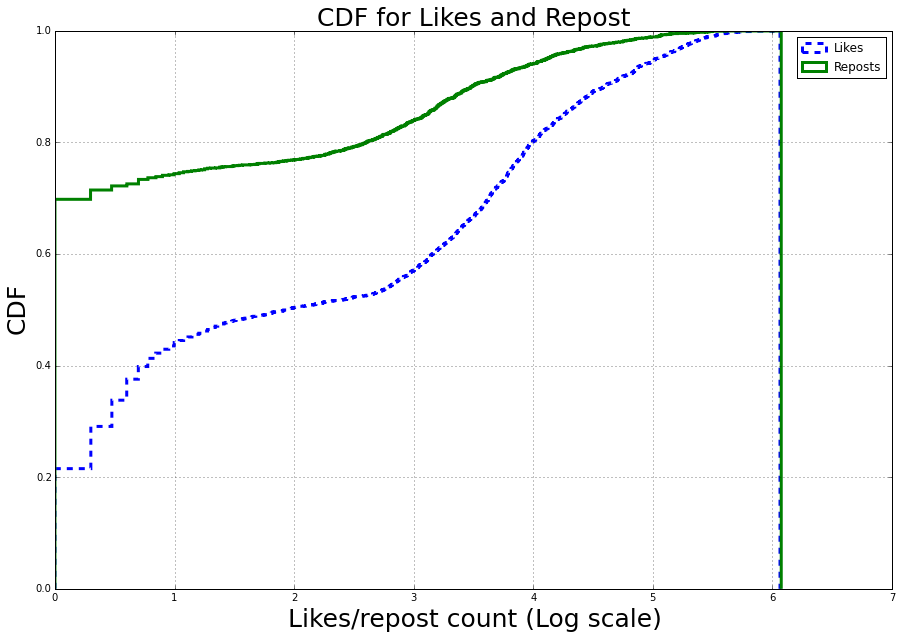
\includegraphics[width=\columnwidth]{plots/CDF_Like_reposts}
\caption{\textsl{ CDF of Like count and Repost count.} \textbf{The values are normalized and on a Logarithmic scale. As expected from a long tail distribution of metrics like popularity, the dataset has a lot of videos with zero likes and reposts. Such videos are synthetically given one like and repost to avoid undefined values}}
\label{fig:CDF_posts}
\end{figure}

Over the course of this study, we also used several third party datasets, to corroborate different properties of vine videos, with datasets previously studied, ranked and evaluated by other research groups. For comparing the aesthetic qualitiy of our videos, we used the dataset provided by Datta et.al \cite{datta2008algorithmic} which provided rated images , rated by a crowdsourced activity, on the scale of 0 to 7. Each image has more than 15 ratings, and the median ratings of these images were considered for our work. 
For our work with frame sentiments, we use the dataset provided by the work of sentibank \cite{jou2015visual} \cite{SentiBank} for baselining the performance of our detector for detecting frame sentiments in vine. Finally for doing the exploratory work with facial expressions, we used the dataset opened up to the public for the facial expression recognition competition 2013 \cite{goodfellow2013challenges} to train and test our convolutional network